%!TEX root = index.tex

\chapter{Flights Scheduling}

\red{TODO}
% že to je zjednodušení problému na 1 rwy
% co je vlastně kritérium
% různé pořadí různých tříd má různé trvání
% popis obrázků plánů
% posun jen doprava ne dřív
% není to project schedulling protože tady to není jednosměrně, když jsou sloty opačně, tak platí jiná podmínka
% nemůžu použít nic z KOčka - popsat co a proč
% nemůžu použít online algoritmy
% většina z nich počítá s tím, že arrival time a release time jsou stejné, u mně jsou různé,
% Shortest processing time first nemůžu použít, protože processing times nejsou konstantní
% není preempce 
%nejde nám o optimální řešení ale good enough které se podobá reálnému řídícímu

\section{Slot Selection}

\red{TODO}
% pokud vede z aktuální pozice jen jedna star, tak stačí plánovat na jedné rwy:

\subsection{Algorithm 1}

\begin{figure}[h]
    \centering
    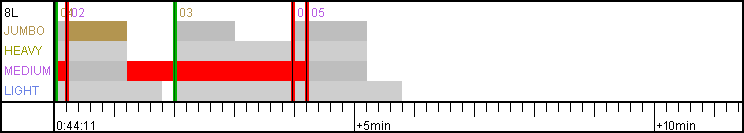
\includegraphics[width=\textwidth]{figures/rwy-in-place.png}
    \caption{Example of runway plan with colliding slots}
    \label{fig:rwy-in-place}
\end{figure}

An example of a plan generated by Algorithm 1 is shown in Figure \ref{fig:rwy-in-place}. This algorithm is the simplest of all implemented, it doesn't perform any deliberation on where to put the slot in the plan and simply places it in the time the aircraft is expected to arrive, ignoring possible collisions with other aircraft. This algorithm is obviously no good for actual use and serves only for comparison to other algorithms and to allow analysing of the traffic flow: it shows how many collisions there are or if the planes arrive to the runway periodically or in groups.

\subsection{Algorithm 2}

\begin{figure}[h]
    \centering
    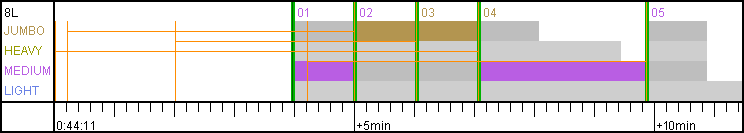
\includegraphics[width=\textwidth]{figures/rwy-end.png}
    \caption{Example of runway with slots in the order of plane's first appearance}
    \label{fig:rwy-end}
\end{figure}

Second algorithm is the simplest one that guarantees no collisions will take place between aircraft. When new plane appears on radar screen it's slot is created after all previously planned slots and not sooner than at the plane's minimal estimated time of arrival.

Figure \ref{fig:rwy-end} shows an example of a plan generated by this algorithm. It is clearly visible that unnecessary delays can occur when the interval between when the plane shows on the radar and its ETA differ from plane to plane. This can happen when the arrival routes have different lengths. Approach route for airplane heading directly to runway will be much shorter than for airplane arriving from opposite direction, because such plane must first fly around the airport before landing. \red{ref to figure with KATL approach routes} In the example shown on Figure \ref{fig:rwy-end} flight \texttt{TRS753} will arrive more than 5 minutes late because it appeared on the radar screen later than flights \texttt{TRS1341} and \texttt{DAL1946}.

\subsection{Algorithm 3}

\begin{figure}[h]
    \centering
    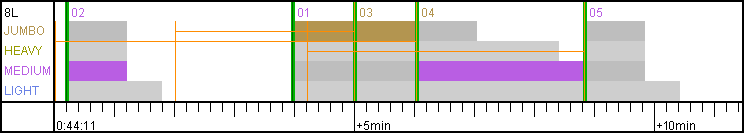
\includegraphics[width=\textwidth]{figures/rwy-fill-voids.png}
    \caption{Example of runway plan with slots fixed in place}
    \label{fig:rwy-fill-voids}
\end{figure}

Algorithm 3 creates the slot for arriving airplane in the first empty space following planes estimated arrival time the slot fits in. The wake turbulence separation minima is taken into account for both preceding and following slot so no collisions between slots occur. The advantage of this this algorithm is its simplicity and the fact that the planed slots are fixed. This means that if the controller assigns a slot to airplane and clears it for approach he/she doesn't have to alter the airplane's clearance and can focus on other arriving aircraft.

An example of a plan generated by Algorithm 3 is shown in Figure \ref{fig:rwy-fill-voids}. In comparison to plan generated by previous algorithm (\ref{fig:rwy-end}) it is apparent that flights \texttt{TRS753}, \texttt{DAL1304} and \texttt{DAL1799} can land sooner than \texttt{TRS1341} even though they entered the controlled area later.

\subsection{Algorithm 4}

\begin{figure}[h]
    \centering
    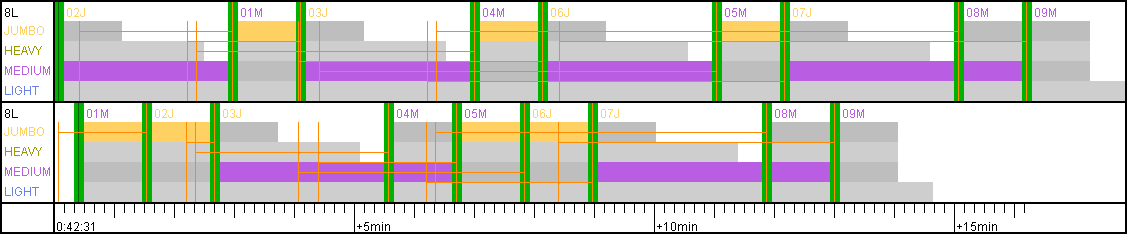
\includegraphics[width=\textwidth]{figures/rwy-eta-order.png}
    \caption{Example of runway plan that preserves the order of estimated time of arrival}
    \label{fig:rwy-eta-order}
\end{figure}

Fourth algorithm was implemented in two variants, the first one schedules the slots in a way that strictly preserves the order of estimated time of arrival. If the slot doesn't fit, any already planned slots following this one are delayed. If there is a continuous string of planes scheduled for approach one after other and new, early arriving plane appears on the radar screen the controller using this algorithm will squeeze the plane in and postpone the planes following in the string. This prevents a situation where the new airplane would wait for all the planes in the string to land first and potentially deplete its fuel supply. On the other hand the controller may need to postpone a significant number of previously planned aircraft which would take a considerable amount of time.

The second variant is not strict with the order according to ETA. It finds the place where the new slot would fit by the ETA, but inserts it only if the delay of the following slot after the new slot is inserted is smaller than the delay of the new slot would be if it was placed after the following slot. Otherwise it tries to insert the new slot after the slot following it and so forth until the condition is met. This serves as a local optimization of the maximal delay and helps the algorithm to cope with flights with alternating weight classes.

The example plans generated by this algorithm are shown in Figure \ref{fig:rwy-eta-order}, first row contains result of first variant, second row contains second variant. First \texttt{01M} was inserted, followed by \texttt{03J}. Then \texttt{02J} arrived with earlier ETA than \texttt{01M}. First variant places the \texttt{02J} to the beginning of the plan and significantly shifts \texttt{01M} and \texttt{03J}. Second variant compares the delay of \texttt{01M} behind \texttt{02J} with delay of \texttt{02J} behind \texttt{01M}. The second delay is smaller and therefore the algorithm doesn't place \texttt{02J} before \texttt{01M}, but continues after \texttt{01M}, here it performs the same comparison between \texttt{02J} and \texttt{03J} and this time placing \texttt{02J} before \texttt{03J}. The algorithm keeps inserting additional slots using this local optimization finally producing much shorter plan than first variant of the algorithm would.

\subsection{Algorithm 5}

\begin{figure}[h]
    \centering
    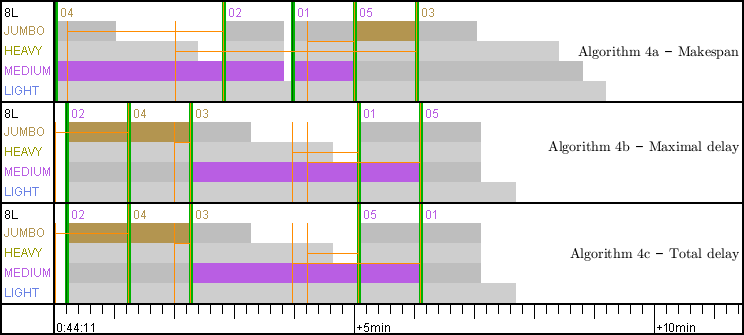
\includegraphics[width=\textwidth]{figures/rwy-bab.png}
    \caption{Comparison between Algorithm 4v1 (first row) and three variants of Algorithm 5}
    \label{fig:rwy-bab}
\end{figure}

Algorithm 5 is an algorithm commonly used in combinatorial optimization and is called Branch and bound. \cite{bab} The algorithm is used here in three different variants, each optimizing different criterion. First variant minimizing $C_{max}$, the schedule length also called makespan, which is equal to completion time of last task.  Second variant minimizes $W_{max} = max\{w_j\}$, maximal waiting time. The waiting time is defined as the difference between release time and start time of the task, in this instance difference between required time of arrival and actual time of arrival. Third variant minimizes $\sum{w_j}$, the sum of all waiting times.

Figure \ref{fig:rwy-bab} shows a comparison between first variant of Algorithm 4 and the three variants of Algorithm 5. The first variant is in the second row, second variant is in the third row and the third variant is in the last row. Note that all three versions perform significantly better than Algorithm 4v1. The difference between the tree variants is small with variant 1 and 3 even producing the exact same plan in this instance.

\begin{figure}[h]
    \centering
    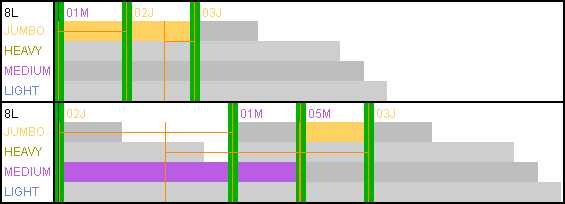
\includegraphics[width=0.7\textwidth]{figures/rwy-proof.png}
    \caption{Example of adding later slot causing changes in plan before its ETA}
    \label{fig:rwy-proof}
\end{figure}

Unfortunately there are two serious problems with Algorithm 5 that prevent its use in real world application.

The first one is that it doesn't keep the relative order of previously planned slots. This is caused by the fact that the algorithm is an offline algorithm and recomputes the whole plan from scratch every time new slot needs to be added. This is illustrated in Figure \ref{fig:rwy-proof} where addition of slot for flight \texttt{05M} caused the order of slots for \texttt{01M}, \texttt{02J} and \texttt{03J} to change. Changing the order of flights scheduled on a route to one runway would result in need of special behaviour that would allow the plane to leave the route, wait in a separate area until the following aircraft flies past on the route and then return back to the route. And because the complete replanning takes place every time new plane appears on a screen it could happen that two flights would switch their place in the sequence back and fort multiple times before reaching runway.

Additionally the planed delay may decrease for any given plane in time (see \texttt{02J} in Figure~\ref{fig:rwy-proof}). But if the plane already performed certain manoeuvre to slow it down to accommodate the delay prescribed by the previous plan, it may be impossible to speed up to reach the runway in time planned by the updated plan, even so it would be able to do so before the hold-up.

\begin{table}[h]
  \centering
\begin{tabular}{ | l || r | r | r | r | r | r | }
\hline
			& 10 slots	& 11 slots	& 12 slots	& 13 slots	& 14 slots	\\
\hline
Version 1	& $< 1s$	& $3s$		& $37s$		& –			& –			\\
Version 2	& $< 1s$	& $< 1s$	& $< 1s$	& $7s$		& $33s$		\\
Version 3	& $< 1s$	& $4s$		& $45s$		& –			& –			\\
\hline
\end{tabular}
  \caption{Run times of the three variants of Branch and bound algorithm}
  \label{tab:alg5-runtime}
\end{table}

The second disadvantage of this algorithm is also linked to the need to recompute the whole plan with each slot addition and it is the computational complexity of the Branch and bound algorithm.

The algorithm enumerates possible solutions in a systematic way that ensures the optimum will be found eventually. To prevent searching through the whole state space, upper and lower bounds are used to prune the unpromising branches from the search tree. The minimal solution found so far can act as an upper bound pruning all branches with partial plans whose criterion value is already bigger or equal to the optimum. This is especially beneficial for the second variant minimizing maximal delay among all slots, because the pruning takes place early on in the search tree, eliminating many non-optimal solutions.

For optimizing makespan any empty voids in the plans can be used as a bound for the solution. This can be done if the slots are ordered according to their ETA. In such case if the ETA of the next added slot is later than the end of the previous slot and forms an empty void before it, the optimal solution lies in a tree rooted by the added slot. This is because rearranging the order of previous slots wouldn't allow the next slot to start sooner than it starts in the current partial solution. This bound cannot be used in variants 2 and 3, because rearranging previously planned slots can still improve maximal and total delay.

The sum of tasks that remain to be planned added to the length to the current partial plan can serve as an upper bound to the solution. If this value exceeds the value of the minimal solution found so far it is obvious that planning the remaining tasks cannot result into better result and current sub-tree can be pruned. This bound cannot be effectively used in this planning problem, because the size of the slots isn't constant and therefore the size of the sum depends on the order in which the slots are added to the plan. And finding the order of the slots that produces the smallest sum equals to the planning problem itself.

The previously mentioned restrictions limit the benefits of pruning and the algorithm must therefore search through a significant part of the state space which makes it slow. The Table \ref{tab:alg5-runtime} shows the runtime for rather small instances of the planning problem and shows that the algorithm can't be successfully used for faster than real time simulation.

\section{Runway Selection}

When the configuration of STARs and the airport allows the planes to land on one of several runways, the air traffic controller must not only decide on the order in which the airplanes land on the runway but also on which plane lands on which runway.

The procedure for runway selection goes as follows: For every runway the arriving plane can land on, new plan is created incorporating the slot for the incoming aircraft. The plans are created using the single-runway algorithms introduced in previous section. Than all the created plans are compared using one of the criteria presented below, the optimal plan is used for the corresponding runway and other plans are thrown away and the runways keep their previous plans not containing the slot of the newly arriving plane.

First criterion used to compare runway plans is ETA of the new slot. The air traffic controller obviously wants the airplanes to land as soon as possible and this criterion is fucused on just that. It compares the arrival times of the newly added slot and directs the airplane to the runway with lowest time. This way the airplane may fly to a runway which is further away if the runway is less utilized and allows for earlier landing than a runway that has the shortest route.

Second criterion guides the airplane to the runway with the smallest makespan after the slot addition. This way the controller keeps all runways equally occupied because new airplane is always routed to the least occupied runway (that is to the one with smallest makespan).

Third and fourth criteria for runway selection are total respectively maximal delay of all slots planned on the runway. The rationale for using these criteria is the same as for planning on single runway mentioned above.

\section{STAR Selection}

Apart from the situation where there are multiple STARs leading to multiple runways, there are also cases where there are multiple routes leading to the same runway leading to the same runway and the air traffic controller must decide which route to use. For example see Figure \red{routy okolo KATL} where airplane arriving from northeast through fix \texttt{FLCON} can land on runway \texttt{9R} flying along either route north of the airport or south of the airport.

The decision is made as follows: when there are multiple routes to one runway arriving flight can take, the one with shortest estimated duration is used for planning. Then schedulling on multiple runways is performed the same way as was described above. If the runway with multiple routes leading to it is selected deliberation on which of the routes to take is carried out. If the slot assigned to the arriving flight has a delay from the ETA of the shortest STAR (because the runway is busy with other flights at the moment) and the delayed ETA is bigger than that of another route with longer duration, this route is used instead of the shortest.

This basically means that if the runway is free, the plane takes the shortest route, but if the flight needs to be delayed, the controller preffers that the plane takes a longer route to take away from the delay rather than hold in one place and taking the short route. The plane needs to be delayed anyway and this way it at least doesn't occupy the holding pattern and instead flies along a different route.